\documentclass{beamer}
\usepackage[russian]{babel}
\usetheme{metropolis}

\usepackage{amsthm}
\setbeamertemplate{theorems}[numbered]

\setbeamercolor{block title}{use=structure,fg=white,bg=gray!75!black}
\setbeamercolor{block body}{use=structure,fg=black,bg=gray!20!white}

\usepackage[T2A]{fontenc}
\usepackage[utf8]{inputenc}

\usepackage{hyphenat}
\usepackage{amsmath}
\usepackage{graphicx}

\AtBeginEnvironment{proof}{\renewcommand{\qedsymbol}{}}{}{}

\title{
Микроэкономика-I
}
\author{
Павел Андреянов, PhD
}

\begin{document}

\maketitle

\section{Тождество Роя}

\begin{frame}{Тождество Роя}

Мы хотим связать между собой три объекта: $x^{\ast}(p,q,I), y^{\ast}(p,q,I)$ и  $V^{\ast}(p,q,I)$. Для этого мы воспользуемся фундаментальным свойством, что косвенная полезность – это полезность, в которую подставили спросы:

$$V(p, q, px + qy) = U(x, y),$$

Убедитесь, что это действительно корректная запись.

Что можно сделать с этим тождеством?
\begin{itemize}
\item продифференциировать по $p$
\item продифференциировать по $q$
\end{itemize}

\end{frame}

%%%%%%%%%%%%%%%%

\begin{frame}{Тождество Роя}

Заметим, что цены входят слева дважды, а справа не входят вообще. То есть с точки зрения дифференциирования по ценам, справа стоит константа, а слева сложная функция. 

По правилам дифференцирования, полный дифференциал функции $V$ по $p$ равен:
\begin{gather*}
\frac{d V}{d p} = \frac{\partial V}{\partial p} + \frac{\partial V}{\partial I} \cdot \frac{\partial I}{\partial p} = 0
\end{gather*}

Поскольку $\frac{\partial I}{\partial p} = x$, 
$$\frac{d V}{d p} = \frac{\partial V}{\partial p} + \frac{\partial V}{\partial I} \cdot x = 0$$

\end{frame}

\begin{frame}{Тождество Роя}

Aналогично для второй цены

$$\frac{d V}{d q} = \frac{\partial V}{\partial q} + \frac{\partial V}{\partial I} \cdot y = 0$$

Комбинируя это в векторной форме, мы получаем:

\begin{theorem}[Тождество Роя]
Если $\vec{x}$ - весь вектор спросов, а $\vec{p}$ - весь вектор цен то
$$\vec{x} = - \nabla_{\vec{p}} V / \nabla_I V$$
\end{theorem}

\end{frame}

\section{Теорема об огибающей}

\begin{frame}{Теорема об огибающей}

Это чрезвычайно важная теорема. Рассмотрим семейство опорных функций $f(x, p)$, где $x$ - переменная а $p$ - параметр. 

Определим огибающую $V(p)$ как результат оптимизации функции $f$ по какому-то статическому множеству $Х$: 
$$ V(p) := \max_{x \in X} f(x, p),$$

\begin{theorem}[Об огибающей]
Функция $V(p)$ дифференциируема (почти всюду) и 
$$\frac{\partial V(p)}{\partial p} = \frac{\partial f(x, p)}{\partial p}|_{x = x^{\ast}(p)}.$$
\end{theorem}

\end{frame}

\begin{frame}{Теорема об огибающей}

... то есть, наклон огибающей равен наклону опорной функции в точке касания.

Представьте себе, что вы сложили вместе крупные предметы разной формы (стол, компьютер, велосипед) и, чтобы они не пылились, накрыли все эластичной пленкой. 

Пленка плотно прилегла к тем предметам, которые оказались, по разным причинам выше всех остальных. Можно сказать, что пленка - это (верхняя) огибающая вашего семейства опорных объектов, поскольку она лежит там, где находится самый высокий объект в каждой точке.

\end{frame}

\begin{frame}{Теорема об огибающей}

\begin{figure}[hbt]
\centering
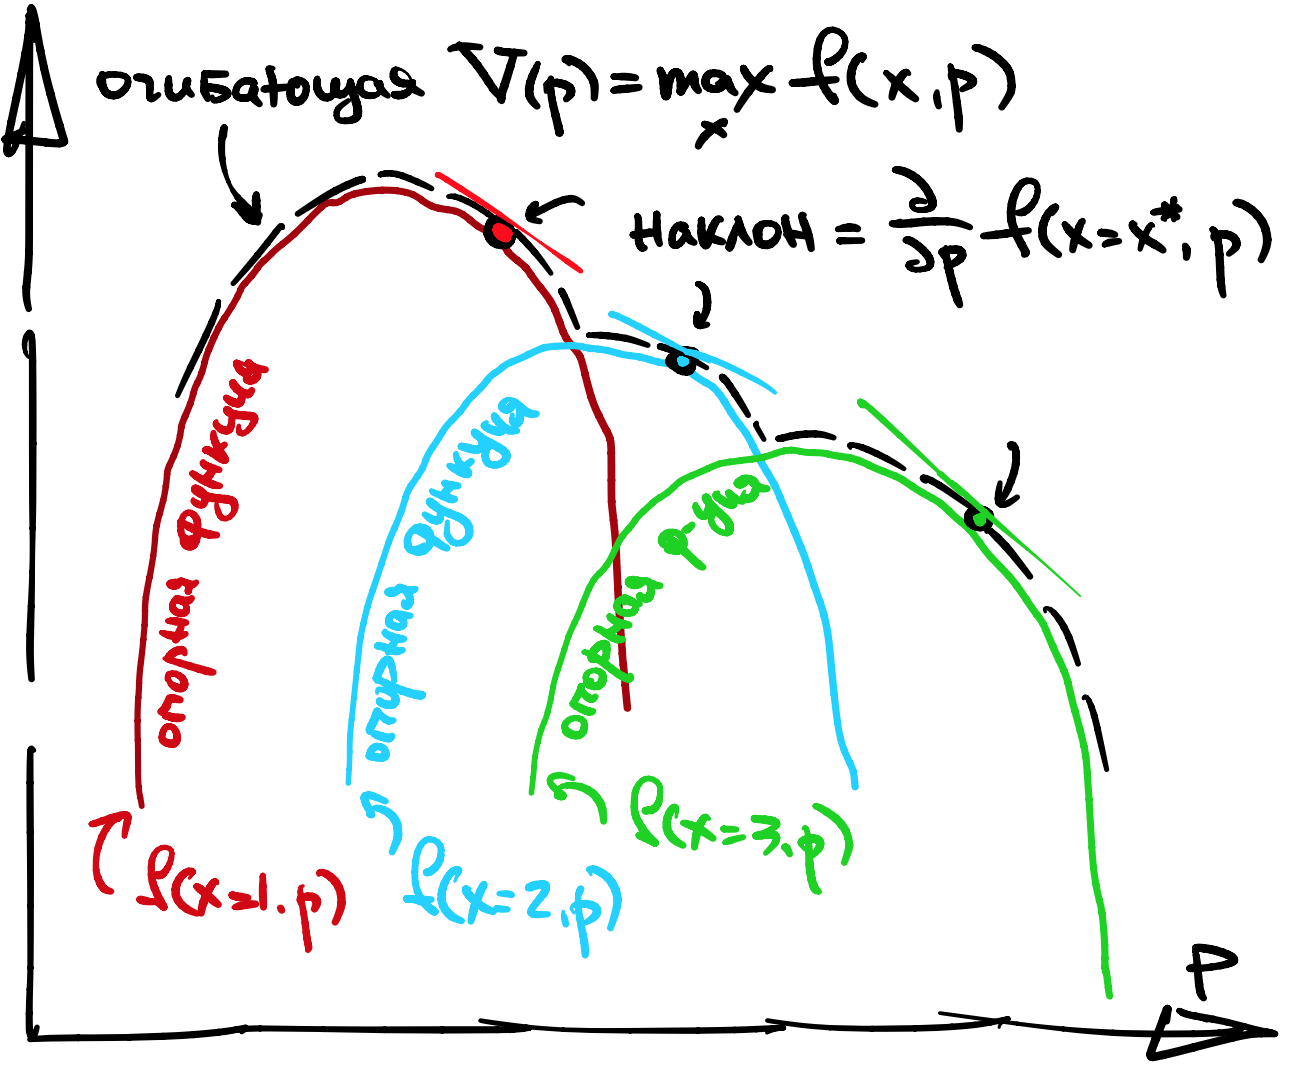
\includegraphics[width=.8 \textwidth]{envelope2.png}
\end{figure}

\end{frame}

\begin{frame}{Теорема об огибающей}

Запомните следующую мантру: 

\textbf{наклон огибающей равен наклону опорной функции в точке касания}. 

То есть, чтобы найти наклон огибающей в точке $p$ нужно из всех опорных функций (они индексированы через $x$) выбрать ту, на которую в этой точке (точка это значение параметра $p$) опирается огибающая, и взять ее наклон, опять же, в пространстве параметра $p$. 

\end{frame}

\begin{frame}{Теорема об огибающей}

Чтобы не перепутать, какие роли $x$ и $p$, помните, что \textbf{огибающая - это функция от параметра}, а не от оптимизационной переменной, которая индексирует опорные функции. 

Соответственно, \textbf{огибание происходит в пространстве парамера, а не в пространстве переменных, по которой вы оптимизировали}.

\end{frame}

\section{Практическая польза}

\begin{frame}{Теорема об огибающей}

Может показаться, что дифференцирование опорной функции и подстановка – это лишняя трата времени, ведь можно просто решить задачу и продифференцировать $V$ по параметру, в лоб.

Это правда, однако если у вас абстрактная функция, вы не можете просто так ее промаксимизировать. Поэтому эта теорема очень удобна при доказательствах, но не только. 

Зачастую видение огибающей позволяет сэкономить время при дифференцировании в том смысле, что вам не надо лишний раз протаскивать производную по правилу дифференциирования сложной функции.

\end{frame}

\begin{frame}{Теорема об огибающей}

К примеру, предположим, что у вас есть функция $F(x, y, p)$ и eще две функции $x = g(p), y = h(p)$. Если вас попросят найти полную производную $F(g(p), h(p), p)$ по $p$ то получится:

$$\frac{d}{dp} F(g(p), h(p), p) = \frac{\partial F}{\partial x} \frac{\partial g}{\partial p} + \frac{\partial F}{\partial y} \frac{\partial h}{\partial p} + \frac{\partial F}{\partial p}.$$

\end{frame}

\begin{frame}{Теорема об огибающей}

Теперь предположим, что нам стало известно, что $x = g(p), y = h(p)$ это, на самом деле, оптимумы функции $F$. 

Тогда, по Теореме об Огибающей

$$\frac{d}{dp} F(g(p), h(p), p) = \frac{\partial F}{\partial p}.$$

Получается, что Теорема об Огибающей позволяет нам \textbf{игнорировать параметр, находящийся внутри оптимальной точки,} при подсчете полного дифференциала.

\end{frame}

\begin{frame}{Теорема об огибающей}

Как насчет косвенной полезности?

Для того, чтобы активировать всю мощь Теоремы об Огибающей, вам достаточно взять любую функцию, которая является результатом оптимизации, и продифференциировать ее по любому параметру.

К примеру, мы могли бы продифференциировать косвенную полезность по ценам. Тогда Теорема об Огибающей даст вам связь этих производных с производными опорной функции в точках оптимума.

\end{frame}

\begin{frame}{Теорема об огибающей}
Чему равна $\partial V/ \partial I$?
\end{frame}

\begin{frame}{Теорема об огибающей}
Она равна множителю Лагранжа $\lambda$.
\end{frame}

\section{Минимизация расходов}

\begin{frame}{Минимизация расходов}
Сейчас мы перейдем к задаче, на первый взгляд, никак не связанной с максимизацией полезности. Если быть точными, мы будем минимизировать сумму расходов на все товары при минимально заданном таргетированном уровне полезности $\bar U$. 

Для простоты пусть будут два товара $x, y$ с ценами $p, q$. 
$$\text{P2:} \quad p x + q y \to \min_{x,y \geqslant 0}, \quad \text{s.t.} \quad U(x,y) \geqslant 0.$$

Сравните с классической задачей максимизации полезности
$$\text{P1:} \quad U(x, y) \to \max_{x,y \geqslant 0}, \quad \text{s.t.} \quad p x + q y \leqslant 0.$$
\end{frame}

\begin{frame}{Минимизация расходов}
Сравним лагранжианы
\begin{gather*}
\mathcal{L}^{1} = U(x, y) - \lambda (px + qy - I)\\
\mathcal{L}^{2} = (px + qy - I) - \gamma (\bar U - U(x,y))
\end{gather*}

Сравним фоки (упп)
\begin{gather*}
\text{P1:} \quad U'_x = \lambda p, \quad U'_y = \lambda q, \quad px + qy = I\\
\text{P2:} \quad p = \gamma U'_x, \quad q = \gamma U'_y, \quad U(x,y) = \bar U
\end{gather*}

Решения совпадают, если третьи уравнения эквивалентны.

Это свойство известно как Закон Вальраса.
\end{frame}

\section{Закон Вальраса}

\begin{frame}{Закон Вальраса}

Для начала приведем пример полезности, при которой Закон Вальраса не выполнен, это постоянная полезность $U(x,y) = 1$. 

Действительно, с точки зрения полезности все бюджетное множество состоит из оптимумов. Однако лишь одна точка $(x,y)=(0,0)$ по настоящему минимизирует издержки, при таргетированной полезности $\bar U = 0$. 

Что тут произошло? Дело в том, что у полезности $U(x,y) = 1$ толстые линии уровня. 

Чтобы Закон Вальраса заработал, необходимо исключить появление таких линий уровня. Это свойство называется локальной ненасыщаемостью в $\mathbb{R}^2_{+}$.

\end{frame}

\begin{frame}{Закон Вальраса}

\begin{definition}
Полезность \textbf{локально ненасыщаема} в $X$, если для каждой точки $x \in X$ и для любой сколько угодно малой окрестности этой точки в $X$, найдется вторая точка $y$ в этой окрестности, такая что $U(y)>U(x)$.
\end{definition}

Большинство полезностей в нашем курсе будет обладать локальной ненасыщаемостью. Теперь мы готовы сформулировать первую теорему

\end{frame}

\begin{frame}{Закон Вальраса}

\begin{theorem}[Закон Вальраса]
Если полезность локально ненасыщаема в $\mathbb{R}^n_{+}$, то любое из решений задачи максимизации полезности всегда лежит на бюджетном ограничении.
\end{theorem}

Это утверждение доказывается от противного. 

Пусть решение находится в бюджетном множестве, но не на бюджетной линии. Тогда существует точка в его окрестности, которая также содержится в бюджетном множестве (поскольку локальная ненасыщаемость именно в $\mathbb{R}^n_{+}$), но дает большую полезность. Противоречие.

\end{frame}

\section{Два спроса}

\begin{frame}{Два спроса}

\begin{definition}
Назовем \textbf{Хиксианским спрос} в задаче минимизации расходов, и \textbf{Маршалианским спрос} в задаче максимизации полезности. 
\end{definition}

Для товаров $x,y$ будем обозначать Хиксианские спросы как 
$$h_x(p,q,\bar U), \quad h_y(p,q,\bar U),$$

а Маршаллианские спросы как
$$m_x(p,q,I), \quad m_y(p,q,I).$$

\end{frame}

\begin{frame}{Два спроса}

Тогда в для задачи максимизации полезности с параметрами $(p,q,I)$ существует 
$$ \bar U_0 := V(m_x(p,q,I), m_y(p,q,I))$$

такой, что задача минимизации расходов с $(p, q, \bar U_0)$ эквивалентна ей. 

Аналогично, для задачи миимизации расходов с $(p, q, I)$ существует
$$ I_0 := p h_x(p,q, \bar U) + q h_y(p,q, \bar U)$$
такой, что задача максимизации полезности с $(p, q, I_0)$ эквивалентна ей. 

\end{frame}

\section{Дуальность}

\begin{frame}{Дуальность}

Мы подошли к очень важному наблюдению.

\begin{theorem}[Дуальность]

Если полезность (квази-)вогнутая и локально ненасыщаемая, то любое решение (как функция от цен) задачи минимизации расходов воспроизводится как одно из решений максимизации полезности и наоборот.
\end{theorem}
Причем, все это при одних и тех же ценах.

\end{frame}

\begin{frame}
Это значит, что задача максимизации полезности и задача минимизации расходов по большому счету эквивалентны в определенном геометрическом смысле. 

Есть только одна проблема - у Маршаллианского и Хиксианского спросов разный набор аргументов, поэтому они не могут совпадать номинально. 

Для того, чтобы поправить ситуацию, нам понадобится еще одна новая функция.
\end{frame}

\section{Функция расходов}

\begin{frame}{Функция расходов}

\begin{definition}
Назовем \textbf{функцией расходов} значение целевой функции в оптимуме в задаче минимизации расходов:
$$ E(p,q,\bar U) = p h_x(p,q,\bar U) + q h_y(p,q,\bar U).$$
\end{definition}

Это совершенно аналогично тому, как мы ввели косвенную полезность $V(p,q,I)$ через значение целевой функции в оптимуме в задаче максимизации полезности.
\end{frame}

\section{Лемма Шепарда}

\begin{frame}{Лемма Шепарда}

Мы проходили сегодня уже Теорему об Огибающей и успешно применили ее к задаче максимизации полезности. А что произойдет, если мы применим ее к задаче минимизации расходов?

$$ E(p,q,\bar U) = p h_x(p,q,\bar U) + q h_y(p,q,\bar U), \quad \frac{\partial E}{\partial p} = ?$$

Прежде всего мы должны ответить на следующий вопрос:
\end{frame}

\begin{frame}{Лемма Шепарда}
Что есть опорная функция для $E(p,q,I)$?
\end{frame}

\begin{frame}{Лемма Шепарда}
Правильный ответ – это Лагранжиан 
$$\mathcal{L}=px + qy - I - \lambda(\bar U - U(x,y)) – $$
это опорная функция.
\end{frame}

\begin{frame}{Лемма Шепарда}
Теперь, когда мы знаем чему равна опорная функция, мы можем сформулировать следующую теорему:
\begin{theorem}[Лемма Шепарда]
Если $\vec{h}$ - весь вектор спросов, а $\vec{p}$ - весь вектор цен то
$$\vec{h} = \nabla_{\vec{p}} E,$$
то есть Хиксианский спрос является градиентом функции расходов.
\end{theorem}
\end{frame}

\section{Как не запутаться?}

\begin{frame}{Как не запутаться?}

Подводя итог, у нас было две задачи: максимизации полезности и минимизации расходов. Каждая задача имела свой набор параметров: первая $(p,q,I)$ а вторая $(p,q,\bar U)$. 

Каждая задача произвела три обьекта:

\begin{itemize}
\item оптимальные $m_x(p,q,I), m_y(p,q,I)$ и косвенная полезность $V(p,q,I)$ в первой задаче
\item оптимальные $h_x(p,q,\bar U), h_y(p,q,\bar U)$ и функция расходов $E(p,q,\bar U)$ во второй задаче
\end{itemize}
Можно изобразить "схему перемещений" между объектами

\end{frame}

\begin{frame}{Как не запутаться?}

\begin{figure}[hbt]
\centering
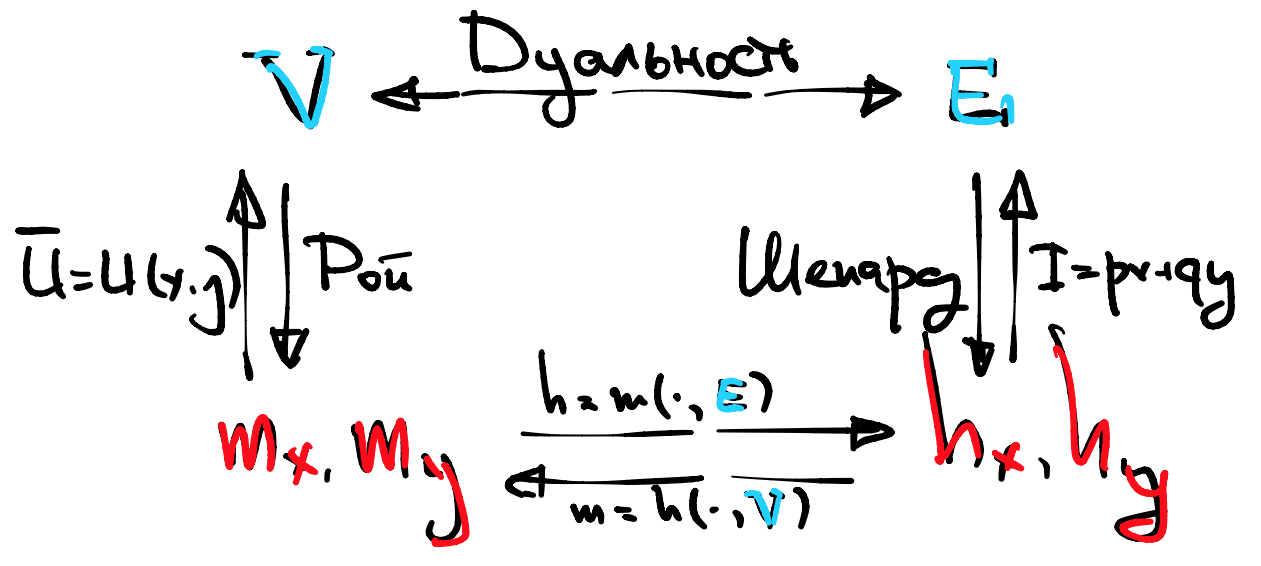
\includegraphics[width=.9\textwidth]{scheme.png}
\end{figure}

\end{frame}

\section{Решаем примеры до упора}

\end{document}